\documentclass[paper=a4, fontsize=11.0pt, abstractoff, DIV12]{scrartcl}
\usepackage[utf8]{inputenc}
\usepackage[ngerman]{babel} % deutsche Rechtschreibung

\usepackage{graphicx} % Grafiken einbinden
\usepackage{amsmath} % AMS! Wichtig!
\usepackage{amsfonts} % mehr AMS
\usepackage{amssymb} % noch viel mehr
\usepackage[amssymb]{SIunits} % Einheiten anständig setzen
\usepackage{bbm} % fetter gedrucktes verfügbar machen, z.B. \mathbbm{1} = Eins mit Doppelstrich
\usepackage{nicefrac}
\usepackage[Euler]{simpleMath}
\usepackage{tikz}
\usepackage{hyperref}
\hypersetup{colorlinks,
            breaklinks=true,
            linkcolor=black,
            urlcolor=black,
            citecolor=black,
            bookmarksnumbered,
            pdfauthor={Alexander Eberspächer},
            pdftitle={Übungen Theoretische Physik}}

\title{Lösungstechniken für partielle Differentialgleichungen I}
\author{Alexander Eberspächer}
\date{\today}

\begin{document}
\maketitle
\begin{abstract}
Um eventuell vorhandene Lücken in der Rechenkunst zu schließen wollen wir kurz
partielle Differentialgleichungen einführen und über Lösungstechniken sprechen.
Ganz ohne jede mathematische Strenge werden so die wichtigsten Begriffe kurz
angerissen. Die Methode der Separation der Variablen wird anhand von Beispielen
etwas detaillierter besprochen.\\[0.5ex]
Literatur: Farlow \cite{Farlow} und Arfken\&Weber \cite{Arfken}.
\end{abstract}

\section{Einführung}

\subsection{Definition}

Eine so genannte \emph{partielle Differentialgleichung} ist eine
Differentialgleichung, in der partielle Ableitungen auftauchen. Ein Beispiel ist
Poissongleichung
\begin{equation}
\left[\secondpderiv{}{x} + \secondpderiv{}{y} + \secondpderiv{}{z}\right] \phi(\vec r) = -\frac{\rho(\vec r)}{\epsilon_0}\, ,
\label{eq:Poisson}
\end{equation}
die den Zusammenhang von elektrischem Potential $\phi$ und Ladungsdichteverteilung
$\rho$ beschreibt.

Weitere Beispiele sind die Schrödingergleichung (in Ortsdarstellung)
\begin{equation}
\left[-\frac{\hbar^2}{2m} \Delta + V(\vec r, t)\right]\psi(\vec r, t) = \ii \hbar\firstpderiv{}{t}\psi(\vec r, t)\,,
\label{eq:SGL}
\end{equation}
die Wellengleichung
\begin{equation}
\left[\frac{1}{c^2}\secondpderiv{}{t} - \Delta\right]\psi(\vec r, t) = 0\,,
\end{equation}
sowie die Maxwell-Gleichungen
\begin{align}
\div \vec E(\vec r, t) &= \frac{\rho(\vec r, t)}{\epsilon_0}\,,\\
\div \vec B(\vec r, t) &= 0\,,\\
\rot \vec E(\vec r, t) &= -\firstpderiv{}{t}\vec B(\vec r, t)\,,\\
\rot \vec B(\vec r, t) &= \mu_0 \vec j(\vec r, t) + \frac{1}{c^2}\firstpderiv{}{t}\vec E(\vec r, t)\,,
\end{align}
ein gekoppeltes System partieller Differentialgleichungen. Die
Hamilton-Jacobi-Differentialgleichung
\begin{equation}
H(\vec q, \vec p=\nabla_{\vec q} S, t) + \firstpderiv{S}{t} = 0
\label{eq:HJ}
\end{equation}
mit $S=S(\vec q, t)$ kennen Sie bereits.

\subsection{Bedeutung}

Partielle Differentialgleichungen sind von so großer Bedeutung, weil wir die
Grundgesetze der Physik als ebensolche Gleichungen schreiben können (Hamilton-Jacobi-DGL, Maxwell-Gl., Schrödinger-Gl., Einsteinsche Feldgl., \dots).

\subsection{Klassifikation}

Es gibt eine Vielzahl von Möglichkeiten, partielle Differentialgleichungen zu klassifizieren, darunter folgende:

\begin{description}
    \item[Ordnung]
    Die Ordnung einer partiellen Differentialgleichung ist die Ordnung der
    höchsten darin auftretenden partiellen Ableitung. Die
    Schrödingergleichung \eqref{eq:SGL} ist also beispielsweise wie die
    meisten Gleichungen von Interesse zweiter Ordnung.
    \item[homogen/inhomogen]
    Taucht neben der gesuchten Funktion (und deren Ableitungen) kein
    weiterer (unabhängiger) Term auf, so nennen wir die Gleichung \emph
    {homogen}, andernfalls ist die Gleichung \emph{inhomogen}. Mit dem
    Differentialoperator $\mathcal{D}$ und der Funktion $f$ schreiben wir
    also \[\mathcal{D}\, f = g\,,\] was für $g=0$ eine
    homogene Gleichung ist und für $g\neq 0$ eine inhomogene Gleichung
    darstellt. Die Poissongleichung \eqref{eq:Poisson} ist beispielsweise
    eine inhomogene Gleichung, falls Ladungen vorhanden sind. Die für
    $\rho(\vec r) = 0$ resultierende homogene Gleichung heißt auch
    Laplace-Gleichung.
    \item[konstante oder veränderliche Koeffizienten]
    Sind die Koeffizienten vor der gesuchten Funktion (und deren Ableitungen)
    alle fest, so spricht man von einer Differentialgleichung mit konstanten
    Koeffizienten, andernfalls spricht man von einer Differentialgleichung
    mit variablen Koeffizienten. Ist in der Schrödingergleichung \eqref
    {eq:SGL} beispielweise das Potential $V(\vec r, t) = \const$, so liegt
    eine Gleichung mit konstanten Koeffizienten vor.
    \item[linear/nichtlinear]
    Treten in einer Gleichung die gesuchte Funktion (und deren Ableitungen)
    nur linear auf, so klassifiziert man die Gleichung als lineare
    Differentialgleichung. Für diese gilt das \emph{Superpositionsprinzip}!
    Ein Beispiel für eine nichtlineare Differentialgleichung ist die
    Gross-Pitaevski-Gleichung
    \begin{equation}
     \left[-\frac{\hbar^2}{2m}{\Delta} + V(\vec{r})  + {4\pi\hbar^2a_s\over m}\vert\psi(\vec{r})\vert^2\right]\psi(\vec{r})=\mu\psi(\vec{r})\,,
    \end{equation}
    die Bose-Einstein-Kondensate beschreibt.\footnote{In diesen kommt in der
    Vielteilchen-Schrödingergleichung neben dem Fallenpotential $V$ noch eine
    Art Hartkugel-Wechselwirkung $c\delta^3(\vec r - \vec r')$ hinzu. Aus
    dieser resultiert in einer sog. ``mean field'' Beschreibung die zur
    Teilchendichte proportionale Nichtlinearität $\abs{\psi(\vec r)}^2$.} Die
    Hamilton-Jacobi-Gleichung \eqref{eq:HJ} ist ebenfalls nichtlinear (die
    Hamiltonfunktion ist quadratisch in $p$!).
\end{description}

\subsection{Randbedingungen}

Ein Problem ist erst dann vollständig beschrieben, wenn neben der
Differentialgleichung auch noch \emph{Randbedingungen} gegeben werden. Die
genaue Form der Randbedingungen folgt aus physikalischen Betrachtungen.
Werden zu einer (linearen) Differentialgleichung mehrere Lösungen gefunden,
so müssen die Lösungen so superponiert werden, dass die Randbedingungen
erfüllt sind.

\subsubsection{Typen von Problemen}

Man unterscheidet oft zwischen
\begin{description}
    \item[Randwertproblemen] Bei diesen Problemen werden die gesuchte Funktion (oder deren Ableitungen) auf dem Rand des Definitionsgebietes vorgegeben.
    \item[Anfangswertproblem] Ist für eine Variable der Definitionsbereich
    offen (zum Beispiel die Zeit $t \in [0; +\infty)$, so spricht man für
    einen am Rand vorgegebenen ``Anfangswert'' auch von einem
    Anfangswertproblem.
\end{description}
Kombiniert spricht man dann von einem ``Anfangs-Randwertproblem''.

\subsubsection{Typen von Randbedingungen}

Es werden auch verschiedene Typen von Randbedingungen unterschieden. Gängig sind

\begin{description}
    \item[Dirichlet-Randbedingungen]
    Bei diesen Randbedingungen wird der Funktionswert auf dem Rand vorgegeben.
    \item[Neumann-Randbedingungen]
    Hier werden Ableitungen vorgegeben. Beispiel: Poissongleichung mit gegebener
    Normalableitung $\dn \phi = f(\vec r)$ auf $\vec r \in \text{Rand}$.\footnote{Die Normalableitung $\dn$ ist definiert als $\dn \circ = \vec n \cdot \grad \circ$, wobei $\vec n$ normal auf der betrachten Fläche steht.
    Sie projiziert also die Normalkomponente aus dem Gradienten. Im Falle eines
    elektrostatischen Potentials $\phi$ ist $\dn \phi = -\vec E \cdot \vec n$
    also parallel zur Normalkomponente des elektrischen Feldes.}
\end{description}
Etwas exotischer sind sicherlich
\begin{description}
    \item[Cauchy-Randbedingungen]
    Cauchy-Randbedingungen mischen Neumann- und
    Dir\-ich\-let-Rand\-be\-ding\-ung\-en so, dass für die gesuchte Funktion $f$ auf
    dem Rand
    \[f(\vec r \in \text{Rand}) = g(\vec r)\quad\text{und}\quad\dn f(\vec r\in \text{Rand}) = h(\vec r)\]
    gelten muss.
    \item[Robin-Randbedingungen]
    Robin-Randbedingungen kombinieren Neumann- und Dir\-ich\-let-Rand\-be\-ding\-ung\-en in
    \emph{einer} Gleichung:
    \[a f(\vec r \in \text{Rand}) + b \dn f(\vec r \in \text{Rand}) = g\,,\]
    wobei $a, b$ und $g$ beliebige auf dem Rand definierte Funktionen sein dürfen.

\end{description}


\section{Lösungstechniken}

Zur Lösung partieller Differentialgleichungen gibt es viele Techniken, zu diesen zählen:

\begin{description}
    \item[Separation der Variablen]
    Diese einfache, aber mächtige Methode führt durch einen geeignet
    gewählten Ansatz eine partielle Differentialgleichung in $n$ Variablen
    auf $n$ gewöhnliche Differentialgleichungen zurück, die sich dann
    leichter lösen lassen. Diese Methode führt oft zum Erfolg, wenn die
    Randbedingungen separabel sind.
    \item[Methode der Greenschen Funktion/``Fundamentallösung'']
    Mit dieser Methode lassen sich inhomogene lineare partielle
    Differentialgleichungen lösen. Die Idee ist hierbei, die Inhomogenität
    in eine Summe aus lauter ``Punktquellen'' zu zerlegen und das Problem
    für \emph{eine} beliebig positionierte Punktquelle zu lösen. Aus der
    Linearität der Differentialgleichung lässt sich dann durch
    Summation/Integration die Lösung für eine \emph{beliebige} Inhomogenität
    zusammenbauen.
    \item[Koordinatentransformationen]
    Durch geeignete Koordinatentransformationen können partielle
    Differentialgleichungen einfacher werden oder gar in gewöhnliche
    Differentialgleichungen zerfallen.
    \item[Integraltransformationen]
    Die Idee hierbei ist, eine Integraltransformation durchzuführen, die das
    Problem vereinfacht. Die Fourier-Transformation beispielsweise macht aus
    einer Ableitung nach der Variable, in der transformiert wird eine
    einfache Multiplikation. Die so erhaltene Gleichung lässt sich nach der
    Transformation lösen und die Lösung in der ursprünglichen Variable durch
    Rücktransformationen gewinnen.
    \item[Numerische Techniken]
    Es gibt für praktisch jedes Problem gut entwickelte numerische Methoden.
    Später im Seminar wollen wir eine davon kennenlernen.
\end{description}
Diese Liste ist nicht vollständig. Im Folgenden wollen wir ein paar Beispiele
rechnen.

\subsection{Separation der Variablen}

Unter der ``Separation der Variablen'' versteht man Ansätze von beispielsweise der Form
\begin{align}
u(\vec r) &= X(x)Y(y)Z(z)\\
\text{bzw.}\quad u(\vec r) &= X(x)+Y(y)+Z(z)
\end{align}
oder
\begin{equation}
u(\vec r, t) = U(\vec r)T(t)\, .
\end{equation}

In diesen Ansätzen wird also die Abhängigkeit von einzelnen Variablen als
Produkt oder Summe von Funktionen in nur einer Veränderlichen ausgedrückt.
Diese Ansätze vereinfachen Probleme oftmals. Drei Beispiele aus der Physik sollen das verdeutlichen. Diese Methode eignet sich besonders, wenn die
Randbedingungen separabel sind. In diesem Fall sind geeigenete Koordinaten zu
wählen.

\subsubsection{Wellengleichung für eine schwingende Saite}

Eine Saite sei bei $x=0$ und $x=L$ fest eingespannt. Die Auslenkung der
Saite am Punkt $x$ zur Zeit $t$ bezeichnen wir mit $\psi(x, t)$.

\begin{center}
    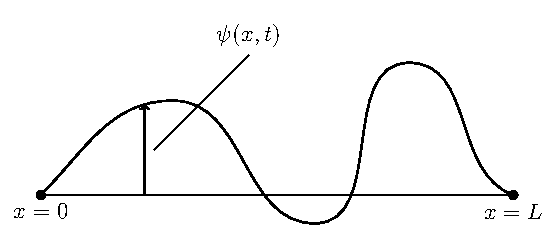
\includegraphics{Figures/Schwing}
\end{center}


Die Wellengleichung in einer Dimension lautet
\begin{equation}
\partial_x^2 \psi(x, t) - \frac{1}{c^2}\partial_t^2 \psi(x,t) = 0\,.
\end{equation}
Wir komplettieren das Problem durch die Randbedingungen
\begin{align}
\psi(x=0,t) &= 0\\
\text{sowie}\quad\psi(x=L,t) &= 0\,,
\end{align}
und die Anfangsbedingungen
\begin{align}
\psi(x,t=0) &= f(x)\, ,\label{eq:AB1}\\
\text{und}\quad\dot{\psi}(x,t=0) &= 0\,.
\end{align}
Die Randbedingungen müssen so gelten, weil die Saite fest eingespannt ist;
die beiden Anfangsbedingungen für Auslenkung und Geschwindigkeit sind
notwendig, weil die Differentialgleichung zweiter Ordnung in der Zeit ist.
Diese ``Anfangs-Randwertaufgabe'' lösen wir nun mit dem Separationsansatz
\begin{equation}
\psi(x,t) = \phi(x)\tau(t)\,,
\end{equation}
mit dem wir Orts- und Zeitabhängigkeit separieren.

Einsetzen des Ansatzes in die Differentialgleichung führt auf
\begin{equation}
\tau \phi'' - \frac{1}{c^2}\phi \tau'' = 0\,,
\end{equation}
oder, nach Division durch $\phi\tau$, auf
\begin{equation}
\frac{\phi''}{\phi} - \frac{1}{c^2}\frac{\tau''}{\tau} = 0\,.
\label{eq:WGL}
\end{equation}
Die Striche stehen für Ableitungen nach dem jeweiligen Argument. Der erste
Summand hängt nur von $x$ ab, der zweite Summand nur von $t$. Die Gleichung
soll für alle $x$ und alle $t$ erfüllt sein, also müssen beide Summanden für
sich konstant identisch der so genannten Separationskonstanten sein! Die
Konstante nehmen wir zunächst als positiv an und schreiben sie als
$+\alpha^2$. Wir haben nun durch die Separation aus einer \emph{partiellen}
Differentialgleichung in zwei Variablen zwei \emph{gewöhnliche} in je einer
Variablen gewonnen! Wir lösen zunächst die Gleichung für die Zeitabhängigkeit,
\begin{equation}
\tau''(t) = +{c^2}{\alpha^2}\tau(t)\,.
\end{equation}
Die Gleichung hat die beiden Lösungen $\tau(t) = \eto{\pm \alpha c t}$. Diese können wir allerdings physikalisch ausschließen, die eine der beiden Lösungen
über alle Maßen wächst.

Wir wählen also die Konstante negativ als $-\alpha^2$.
Die Gleichung
\begin{equation}
\tau''(t) = -{c^2}{\alpha^2}\tau(t)
\end{equation}
hat die Lösung
\begin{equation*}
\tau(t) = A\sin\left({c}{\alpha} t\right) + B\cos\left({c}{\alpha} t\right)\,,
\end{equation*}
die wir mit $\omega := {c}{\alpha}$ als
\begin{equation}
\tau(t) = A\sin\left(\omega t\right) + B\cos\left(\omega t\right)\,,
\end{equation}
notieren.

Analog dazu ist die Lösung zu
\begin{equation}
\phi''(x) = -\alpha^2\phi(x)
\end{equation}
gleich
\begin{equation}
\phi(x) = C\sin\left({\alpha} x\right) + D\cos\left({\alpha} x\right)\,.
\end{equation}

Mit den Randbedingungen bestimmen wir nun die Lösungen etwas genauer.
Aus $\psi(x=0, t) = \psi(x=L, t) = 0$ folgt
\begin{align}
D &= 0\,,\\
\alpha &= \frac{\pi m}{L}\qquad m \in \Naturals\, .
\end{align}
Wir definieren $k_m:=\alpha_m=\pi m/L=\omega/c$.\footnote{Den Zusammenhang zwischen
Wellenzahl $k$ (``Frequenz im Ort'') und Frequenz $\omega$ (``Frequenz in
der Zeit'') nennt man auch Dispersionsrelation -- diese ist hier linear, $\omega = ck$.}
Für jedes $m$ haben wir dann also eine Lösung
\begin{equation}
\psi_m(x,t)=\phi_m(x)\tau_m(t) = \left[A_m\sin\left(\omega_m t\right) + B_m\cos\left(\omega_m t\right)\right]C_m\sin\left(k_m x\right)
\end{equation}

Weiterhin muss auch $\dot{\psi}(x,t=0) = 0$ gelten, woraus
\begin{equation}
A_m = 0
\end{equation}
folgt. Mit einer weiteren Abkürzung $E_m := B_m C_m$ bleibt also für festes $m$
\begin{equation}
\psi_m(x,t)= E_m\cos\left(\omega_m t\right)\sin\left(k_m x\right)\,.
\end{equation}
Wir müssen nun alle Lösungen für verschiedene $m$ so superponieren, dass die
Anfangsbedingung \eqref{eq:AB1} erfüllt ist. Die allgemeine Lösung ist also
\begin{equation}
\psi(x,t)= \sum\limits_{m=1}^{+\infty}E_m\cos\left(\omega_m t\right)\sin\left(k_m x\right)\,.
\label{eq:WGlsg}
\end{equation}

Um nun die $E_m$ aus der Anfangsbedingung \eqref{eq:AB1} zu bestimmen,
erinnern wir uns an
\begin{equation}
\int\limits_{0}^{L} \sin\left(\frac{\pi n}{L}x\right) \sin\left(\frac{\pi m}{L}x\right)\,\dd x = \frac{L}{2} \delta_{mn}\,.
\end{equation}
was eine Orthogonalitätsrelation ist.\footnote{Die Sinusfunktionen sind für
Indizes $m\ne n$ auf dem Intervall $[0;L]$ orthogonal.} Wir nutzen diese
Relation nun zusammen mit \eqref{eq:WGlsg} in \eqref{eq:AB1} aus -- dazu
multiplizieren wir die Gleichung mit $\sin\left(\frac{\pi n}{L}x\right)$ und
integrieren über die Saite. Es ergibt sich\footnote{Summation und
Integration dürfen vertauscht werden.}
\begin{align}
\int\limits_{0}^{L}\psi(x,t=0)\sin(k_n x)\,\dd x &= \sum\limits_{m=1}^{+\infty}E_m\int\limits_{0}^{L}\sin(k_m x)\sin(k_n x)\,\dd x\nonumber\\
&= \sum\limits_{m=1}^{+\infty} E_m \frac{L}{2} \delta_{nm}\nonumber\\
&=\frac{L}{2}E_n\,.
\end{align}
Die Koeffizienten $E_m$, die unsere Lösung \eqref{eq:WGlsg} der Anfangsbedingung
genügen lassen sind also durch
\begin{equation}
E_m = \frac{2}{L}\int\limits_{0}^{L}\psi(x,t=0)\sin(k_m x)\,\dd x
\end{equation}
bestimmt.

Man beachte den engen Zusammenhang unserer Lösung mit Fourier-Reihen. Wir
haben kein Wissen zu Fourierreihen vorausgesetzt, sondern nur die
Orthogonalität der Sinusfunktionen verwendet -- und trotzdem finden wir,
dass die Lösung genau über eine Fourierzerlegung der Anfangsauslenkung zu
erhalten ist. Eine ähnliches Endergebnis werden wir im nächsten Abschnitt
finden.

Zur Wahl des Vorzeichens der Separationskonstante sei gesagt, dass bei
Differentialgleichungen des betrachteten Typs das Vorzeichen entweder
oszillierendes oder exponentielles Verhalten führt.

\subsubsection{Laplace-Gleichung für einen Kreis}

Zu lösen sei die zweidimensionale Laplace-Gleichung
\begin{equation}
\left[\secondpderiv{}{x} + \secondpderiv{}{y}\right] \phi(x,y) = 0
\end{equation}
mit der Randbedingung, dass $\phi$ auf dem Einheitskreis $r=1$ durch
\begin{equation}
\phi(r=1, \theta) = u(\theta)
\label{eq:LaplaeRB}
\end{equation}
gegeben ist.

Die Symmetrie der Randbedingung spricht hier für die Verwendung von
Polarkoordinaten. Der Laplaceoperator in ebenen Polarkoordinaten $(r, \theta)$ ist
\begin{equation}
\Delta = \secondpderiv{}{r}+\frac{1}{r}\firstpderiv{}{r} + \frac{1}{r^2}\secondpderiv{}{\theta}\,.
\end{equation}
Hier ist schon ersichtlich, dass die zu lösende Gleichung variable Koeffizienten
haben wird -- die Gleichung wird allerdings separabel sein!

Der Separationsansatz $\phi = \phi(r,\theta) = R(r)\Theta(\theta)$ führt auf
\begin{equation}
\Theta R'' + \frac{1}{r}\Theta R' + \frac{1}{r^2} R\Theta'' = 0\, ,
\end{equation}
oder -- nach Multiplikation mit $r^2/\Theta R$ auf
\begin{equation}
\underbrace{r^2 \frac{R''}{R} + r\frac{R'}{R}}_{=+\alpha^2} = - \underbrace{\frac{\Theta''}{\Theta}}_{=-\alpha^2}\,.
\end{equation}
Das Vorzeichen des Separationskonstante wurde hier schon so gewählt, dass
die Lösung periodisch in der (periodischen) Koordinate $\theta$ sein wird.
Wir haben also durch eine ähnliche Vorgehensweise und ähnlicher
Argumentation wie im vorigen Abschnitt wieder zwei \emph{gewöhnliche}
Differentialgleichungen gewonnen:
\begin{align}
\Theta''(\theta) + \alpha^2 \Theta(\theta) &= 0\\
r^2 R''(r) + r R'(r) - \alpha^2 R(r) &= 0
\end{align}
Die erste Gleichung wird gelöst von
\begin{align}
\Theta(\theta) &= A\eto{\pm \ii \alpha \theta}\nonumber\\
\text{beziehungsweise}\qquad \Theta(\theta) &= A_1\sin(\alpha \theta) + A_2\cos(\alpha\theta)\,,
\end{align}
woraus wir eine Ausage über $\alpha$ gewinnen. Weil aufgrund der
Symmetrie des Problems die Lösung $2\pi$-periodisch sein muss, also
\begin{equation}
\Theta(\theta + 2\pi) = \Theta(\theta)
\end{equation}
gelten muss, kann $\alpha$ nur eine ganze Zahl sein. Damit und mit der
speziellen Form der Gleichung für $R$ ($r^n$ vor $n$-ter Ableitung)
motiviert sich ein Potenzansatz für $R(r)$. Mit $R(r) = br^n$ finden wir durch
einsetzen
\begin{align}
r^2 n(n-1)r^{n-2} + r n r^{n-1} - \alpha^2 r^n &= 0\nonumber\\
\Leftrightarrow\quad (n^2 -n +n)r^n - \alpha^2 r^n &= 0\,,
\end{align}
woraus wir $n=\pm\alpha$ ablesen. Von der Superposition
\begin{equation}
R(r) = br^{+\alpha} + cr^{-\alpha}
\end{equation}
können wir allerdings nur den ersten Term berücksichtigen, da der zweite Term
für $r\to0$ divergiert. Zusammengefasst haben wir nun die Lösungen
\begin{equation}
\phi_n(r, \theta) = r^n\left[E\sin(n\theta) + F\cos(n\theta)\right]\,,
\end{equation}
wobei Konstanten zusammengeführt wurden. Diese Lösungen müsste man jetzt so
superponieren, dass die Randbedingung \eqref{eq:LaplaeRB} erfüllt ist. Wenn
man das Potential auf dem Rand in eine Fourierreihe zerlegt bedarf es dafür
nicht mehr als einen Koeffizientenvergleich!

\subsubsection{Von der zeitabhängigen Schrödingergleichung zur zeitunabhängigen Schrödingergleichung}

Die Schrödingergleichung für ein zeitunabhängiges Potential $V=V(\vec r)$ lautet
\begin{equation}
\underbrace{\left[-\frac{\hbar^2}{2m} \Delta + V(\vec r)\right]}_{:=\hat{H}}\psi(\vec r, t) = \ii \hbar\firstpderiv{}{t}\psi(\vec r, t)\,.
\label{eq:SGLII}
\end{equation}
Der Operator $\ii\hbar\partial_t$ auf der rechten Seite ist dabei der Energie-Operator $\hat{E}$, der der Eigenwertgleichung
\begin{equation}
\hat{H}\psi(\vec r, t) = \hat{E}\psi(\vec r, t) = E \psi(\vec r, t)
\end{equation}
genügen muss. Der Ansatz $\psi(\vec r, t) = \phi(\vec r)\tau(t)$ führt dann auf
\begin{equation*}
\phi(\vec r) \ii \hbar \partial_t \tau(t) = \phi(\vec r) E \tau(t)
\end{equation*}
beziehungsweise auf
\begin{equation}
\phi(\vec r) \left[\ii \hbar \partial_t \tau(t) - E \tau(t)\right]=0\,,
\end{equation}
was nach dem Satz vom Nullprodukt für alle Lösungen der \emph{gewöhnlichen}
Differentialgleichung
\begin{equation}
\tau'(t) = -\frac{\ii}{\hbar}E\tau(t)
\end{equation}
erfüllt ist. Die Lösung dieser Gleichung ist
\begin{equation}
\tau(t) = \eto{-\ii E t/\hbar}\,.
\end{equation}
Setzt man das in \eqref{eq:SGLII} ein, so erhält man die \emph{zeitunabhängige} Schrödingergleichung
\begin{equation}
\left[-\frac{\hbar^2}{2m} \Delta + V(\vec r)\right] \phi(\vec r) = E\phi(\vec r)\,,
\end{equation}
die natürlich leichter zu lösen ist als die zeitabhängige Version dieser
Gleichung. Die Gesamtlösung $\psi(\vec r, t) = \phi(\vec r) \eto{-\ii E t/\hbar}$
hat also eine zur Zeit proportionale Phase.

\nocite{*}

\bibliographystyle{ieeetr}

\bibliography{EDyn-PDE}

\end{document}
